\chapter{Introduction} \label{chp1}

This chapter gives an overview of joint modeling and motivations of this dissertation. Additionally, we explain the Bayesian hierarchical model and illustrate an example analyzed by Stan via Hamiltonian Monte Carlo (HMC).  

\section{Background}
\subsection{Joint Model}

In many clinical or epidemiological research studies, the longitudinal data may be censored by a time-to-event outcome, such as death or dropout. In order to explore how changes in the biomarker are associated with the occurrence of the terminal event, joint modeling of longitudinal and survival data has became to be prevailing (\cite{Tsiatis2004}, \cite{Henderson2000}, \cite{Rizopoulos2012}, \cite{Ibrahim2010}, \cite{Wulfsohn1997}, \cite{Asar2015}). 

It was summarized in three main features for its popularity (\cite{Hickey2016}):

\begin{enumerate}
    \item Improving inference for a repeated measurement outcome subject to an informative dropout mechanism;
    \item Improving inference for a time-to-event outcome, whilst taking account of an intermittently error-prone measured endogenous time-dependent variable;
    \item Studying the relationship between the two correlated processes
\end{enumerate}
Generally, a joint model with shared parameter refers to the simultaneous estimation of a longitudinal outcome characterized by a linear mixed effects (LME) submodel and a terminal event subject to a survival or time-to-event submodel. The longitudinal and time-to-event submodels are linked using shared individual-specific parameters, which can be parameterised in a number of ways, such as random effects (see Chapter \ref{chp2}), current value (see Chapter \ref{chp3}), time-dependent slope (see Chapter \ref{chp3}), cumulative effects, lagged time, etc.      

% Joint estimation of these two submodels is achieved by assuming an association structure.
\subsection{Extended Joint Model}

The joint model has focused on modeling a single longitudinal outcome and a single time-to-event outcome; thereby known as univariate joint modeling. Nonetheless, a vast number of extensions have been proposed to increase the flexibility for complicated studies, such as latent class joint model (\cite{Proust-Lima2014}), competing risks (\cite{Andrinopoulou2017}), recurrent events (\cite{Krol2016}, \cite{Hickey2018}, \cite{Ren2021}), multiple longitudinal outcomes (\cite{Musoro2015}), accelerated failure time (\cite{Luo2014a}), longitudinal binary outcomes (\cite{Horrocks2009}). Among those extensions, we are interested in joint model for binary outcomes (see Chapter \ref{chp2}) and joint model for time-to-recurrent events (see Chapter \ref{chp3}) given the feature of our motivating data. Moreover, joint modeling has been demonstrated to improve the prediction (\cite{Rizopoulos2014}). Our prognostic rationale is primarily based on inherently Bayesian-frequentist approach in Chapter \ref{chp2} and 
predictive posterior distribution incorporated with Monte Carlo method in see Chapter \ref{chp3}. 

% However, in practice, the data will be often complicated, issuing possible multiple biomarkers and binary outcomes or recurrent or competing event times. Therefore a vast number of extensions have been proposed over the past two decades. 

% The book of Rizo2012 has a comprehensive guidance for possible extensions, such as stratified relative risk models, latent class joint model, multiple failure times, accelerated failure time models, joint models for categorical 
% longitudinal outcomes, joint models for multiple longitudinal outcomes, ect. 
\subsection{Parameter Estimation}

Frequentist and Bayesian estimations are utilized as two widespread approaches to manage technical and computational challenges from aforementioned joint models. The Bayesian statistics is older than frequentist statistics, but it has been neglected over the years due to computer technologies and discovery of new mathematical methods (\cite{Hackenberger2019}). 

A class of algorithms from notion of Markov Chain Monte Carlo (MCMC) (\cite{Metropolis1953}, \cite{Hastings1970}, \cite{Geman1984}, \cite{Tanner1987}, \cite{Gelfand1990}, \cite{Geyer1992}, \cite{Tierney1994}) initiated the era of modern Bayesian approach, which offers insight into estimating from posterior probability density functions that are not analytically tractable. For a comprehensive treatment of MCMC techniques, we defer readers to the handbook of MCMC (\cite{handbook2011}). Furthermore, Bayesian statistics incorporates the ease of hierarchical models, such as employed in \cite{Luo2014} and \cite{Brilleman2019}. Consequently, main methodologies addressed in this dissertation are in Bayesian perspective, however, we adapt to frequentist approach as appropriate.

\subsection{Computation}

A number of packages from mainstream statistical softwares, including R (\cite{R2020}), SAS (SAS Institute, Cary, NC), Stata (Stata-Corp LP, College Station, TX) and WinBUGS (MRC Biostatistics Unit, Cambridge, UK), have allowed researchers to well exploit joint modeling (\cite{Hickey2016}). In this dissertation, we primarily use with R. A recently released R package named \emph{JMBayes2} (\cite{Rizopoulos2022}) is powerful in fitting extended joint models via MCMC implemented in C++. Another Bayesian user-friendly R package named \emph{rstanarm} utilizes Stan (\cite{Goodrich2020}) for the back-end estimation. The convenient \emph{stan\_jm} function allows for univariate or multivariate joint model with avoidance of writing own Stan programs (\cite{Brilleman2018}). Despite the robustness of existing packages, we implement our own R codes along with Stan programs in terms of our particular needs, which will be described in details in the following chapters of this dissertation. 


\section{Motivation}

The motivation of this dissertation arises from the personalized prediction of pulmonary exacerbation (PE) risk in a epidemiological study of United States Cystic Fibrosis Foundation Patient Registry. In order to monitor progressive changes of lung function in people living with cystic fibrosis (CF), a variety of measures and outcomes are collected at each patient’s clinical visit. Typically, a primary longitudinal marker named \emph{percent predicted forced expiratory volume in 1 second} (hereafter, ppFEV1), is commonly used to describe the severity of lung disease. This continuous outcome is obtained from Global Lung Initiative Equations based on observed FEV1 in liters (\cite{Quanjer2012}). Whilst the binary event PE is defined by a recorded antibiotics treatment during hospitalization. One inconceivable feature for our registry data is of three-level hierarchical structure, which is displayed in Figure \ref{chp1_hds}; longitudinal measurements of the biomarker ppFEV1 and PE events are observed at time points (level 1 of the hierarchy), which are clustered within patients (level 2 of the hierarchy), who come from local CF centers (level 3 of the hierarchy). For this cause, we are motivated to propose a multilevel Bayesian joint model to study the underlying associations between the two processes of ppFEV1 and PE. Specifically, we regard PE as a binary longitudinal outcome in Chapter \ref{chp2}, while a time-to-recurrent event in Chapter \ref{chp3}.   

\begin{figure}[H]
\centering
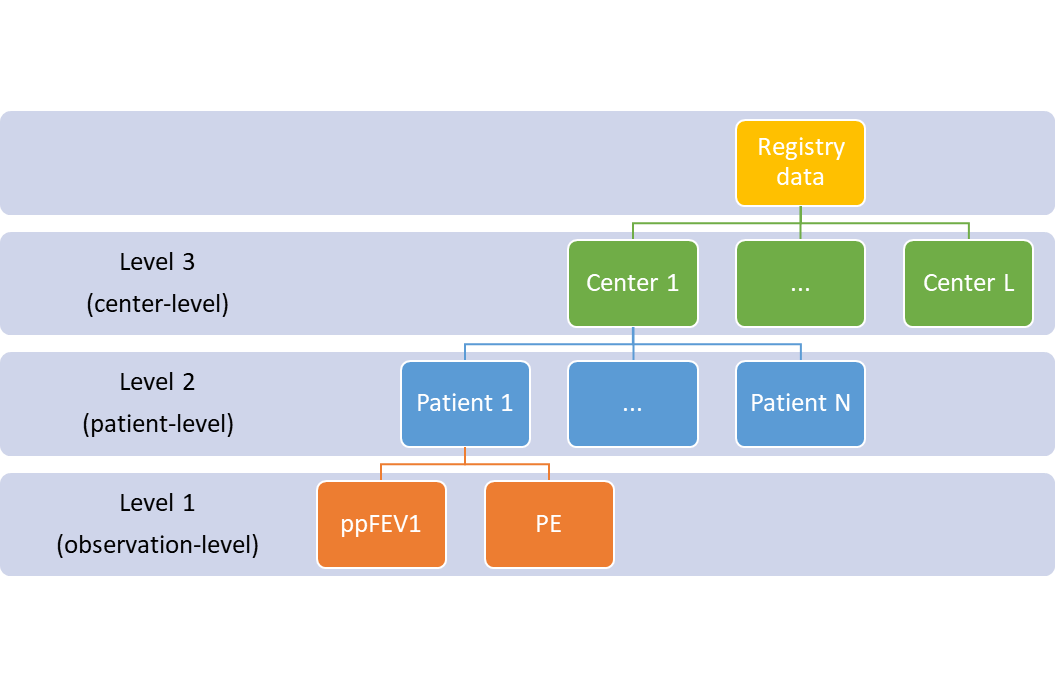
\includegraphics[width=\textwidth]{Figures/Chp1_HDS.png}
\caption{Example of the hierarchical structure of CF registry data}
\label{chp1_hds}
\end{figure}


\section{Hierarchical Model}

Throughout this dissertation, we borrow the key idea of the hierarchical (multilevel) model, allowing for observable outcomes being modeled conditionally on certain parameters, which themselves are given a probabilistic specification in terms of further parameters, known as hyperparameters. Hierarchical concept helps in understanding multiparameter problems and also plays an important role in developing computational strategies. More importantly, simple nonhierarchical models are usually inappropriate for hierarchical data. (\cite{Gelman2013a})


\subsection{Bayesian Inference}

Let $\bm{\theta}$ denote unknown parameters with $\bm{\phi}$ as the corresponding hyperparameters and $\bm{y}$ represent observed data. The key 'hierarchical' part is that $\bm{\phi}$ is unknown and thus has its own prior distribution, $p(\bm{\phi})$. The joint posterior distribution is given by 

\begin{align}
    p(\bm{\theta, \phi}|\bm{y}) & \propto p(\bm{y}|\bm{\theta,\phi})p(\bm{\theta,\phi}) \\
    & =\underbrace{p(\bm{y}|\bm{\theta})}_\text{likelihood} \underbrace{p(\bm{\theta}|\bm{\phi})}_\text{1st-stage prior} \underbrace{p(\bm{\phi})}_\text{2nd-stage prior} \nonumber
\end{align}
with the latter simplification holding because data distribution depends only on $\bm{\theta}$. The prior distribution for $\bm{\phi}$ relies on its extent of uncertainty. Either diffuse prior or (weakly) informative prior can be utilized, however, we should ensure the resulting posterior distribution is proper when using an improper prior density. More details of prior choice recommendations defer to Gelman's post(\cite{Gelman2020}). 


\subsection{Hamiltonian Monte Carlo}

Although the primary implementation is on the ubiquitous stochastic MCMC methods, in particular Metropolis-Hastings (\cite{Hastings1970}) and Gibbs sampling (\cite{Gelfand1990}), Betancourt and Girolami (\cite{Betancourt2013}) introduced a sophisticated but novel MCMC techniques, which is well known as Hamiltonian Monte Carlo (\cite{Neal2011}). It utilizes techniques from differential geometry to generate transitions spanning the full marginal variance, eliminating the random walk behavior endemic to Random Walk Metropolis and the Gibbs samplers, therefore, provides the efficient exploration for the complex hierarchical models. Detailed algorithms are not included here due to the distraction from our main purpose. Readers can refer to the Section 3 of their paper for theoretical interests.  

% The usual way to model exchangeability with covariates is through conditional independence: $p(\theta_1,\dots,\theta_j|x_1,\dots,x_J)=\int\big[\prod_{j=1}^{J}p(\theta_j|\phi,x_j)\big]p(\phi|x)d\phi$. 

% The joint prior distribution is 

% \begin{align}
%     p(\bm{\phi,\theta})=p(\bm{\theta}|\bm{\phi})p(\bm{\phi})
% \end{align}
% and the joint posterior distribtuion is 

% \begin{align}
%     p(\phi,\theta|y) & \propto p(y|\phi,\theta)p(\phi,\theta) \\
%                      & = p(y|\theta)p(\phi,\theta) \nonumber
% \end{align}

\subsection{Stan}

The inference engine Stan (not an acronym; \cite{StanManual}) releases computational constraints of Euclidean HMC. Users can build, test and run hierarchical models through this powerful probabilistic programming language for specifying the target function. Particularly, Stan adapts to No-U-Turn Sampler to preserves detailed balance by integrating not just forward in time but also backwards (\cite{Hoffman2011}). 

% overcome sensitivity to tuning parameter caused by HMC.  

In this section, we illustrate an example of hierarchical model in Stan through the combinations of two interfaces and two methods of parameterizations (centered and non-centered). Specifically, the interfaces to Stan are described as a new lightweight interface named \emph{CmdStanR}(\cite{Gabry2022}) and the conventional interface named \emph{RStan} (\cite{Rstan2020}). Note that in order to execute \emph{CmdStanR}, it is necessary to install \emph{CmdStan} first. Then we consider the Eight Schools example (\cite{Rubin1981}) in terms of the centered parameterization (\cite{Betancourt2017}), 

\begin{gather*} 
    y_n \sim N(\theta_n, \sigma_n)\\
    \theta_n \sim N(\mu, \tau)\\
    \mu \sim N(0,5) \\
    \tau \sim \mbox{Half-Cauchy}(0,5)
\end{gather*}
where $n \in \{1,\dots,8\}$ and $\{y_n, \sigma_n\}$ are given data. Secondly,  with respect to the non-centered parameterization, we introduce a latent Gaussian variable from which we can recover the group-level parameters with a scaling and a translation,

\begin{gather*} 
    y_n \sim N(\theta_n, \sigma_n)\\
    \Tilde{\theta} \sim N(0,1)\\
    \mu \sim N(0,5) \\
    \tau \sim \mbox{Half-Cauchy}(0,5)\\
    \theta_n = \mu + \tau \cdot \Tilde{\theta}
\end{gather*}

In practice, we have the same setup for the four scenarios, for instance, seed=2022, adapt\_delta=0.8, max\_treedepth=10, chains=2, warmup=1000, iters=2000. The Stan programs and R code are included in Appendix \ref{app:a}. From Figure \ref{fig:chp1_mean_tau}, we observe that resulting mean of $log(\tau)$ is strongly biased away from the true value for centered parameterization. Nonetheless, the pathology of bias and divergence is well solved by non-centered method and a thorough discussion of the non-centered intuition can be found in \cite{Betancourt2015}. It is worth noting that both interfaces are supposed to bear the same results as long as all inputs are the same. In this motivating example, we allow initial values to be unassigned so that each trajectory is distinguishable and we aim to compare elapsed time and system compatibility rather than doubting the estimates. 

Figure \ref{fig:chp1_trace_tau} shows the chains from centered parameterization (left panel) are sticking as they approaches negative values of $log(\tau)$ (or small values of $\tau$), which is indicative of the divergences. On the contrary, non-centered parameterization (right panel) stretches $log(\tau)$ further towards negative values and shows the capability to explore the neck of the funnel.

To the end, we apply the superior non-centered trick to our proposed joint models in Chapter \ref{chp2} \& \ref{chp3}. Besides, we confirm less elapsed time by interface \emph{CmdStanR}, although such advantage is not obvious in the formal example. However, when we have complicated model setups and larger sample size, the efficiency will be easily observed (see Appendix \ref{app:b}). We also note that \emph{RStan} is more compatible to windows system, while \emph{CmdStanR} is more favorable to macOS system. For applications, \emph{RStan} is utilized in Chapter \ref{chp2} while \emph{CmdStanR} is included in Chapter \ref{chp3}. To access the accuracy of posterior mean estimation, equal-tailed credible intervals are employed. Notwithstanding 95\% credible interval (CI) from \emph{RStan} is common, 90\% posterior uncertainty intervals from \emph{CmdStanr} are also recommended due to more computational stability and relation to Type-S errors (\cite{Gelman2014b}). Both intervals are incorporated in our dissertation, whilst taking account of a simulation study with $S$ replicates, we compute its corresponding 95\% confidence interval for an averaged posterior mean estimate, that is $\bar{\theta} \pm z_{0.025} * \frac{\sqrt{\sum_{s=1}^{S}(\hat{\theta}_s-\bar{\theta})^2/(S-1)}}{\sqrt{S}}$ with $\bar{\theta}=\frac{\sum_{s=1}^{S}\hat{\theta}_s}{S}$.  

%funnel of hell problem in hierarchical model
% The benefit from the non-centered parameterization is evident from Figure X. Particularly, we pick one parameter $\tau$ and transform into its logarithm $log(\tau)$. Because the logarithm allows us to better resolve behavior for small values.   

\begin{figure}[H]
\centering
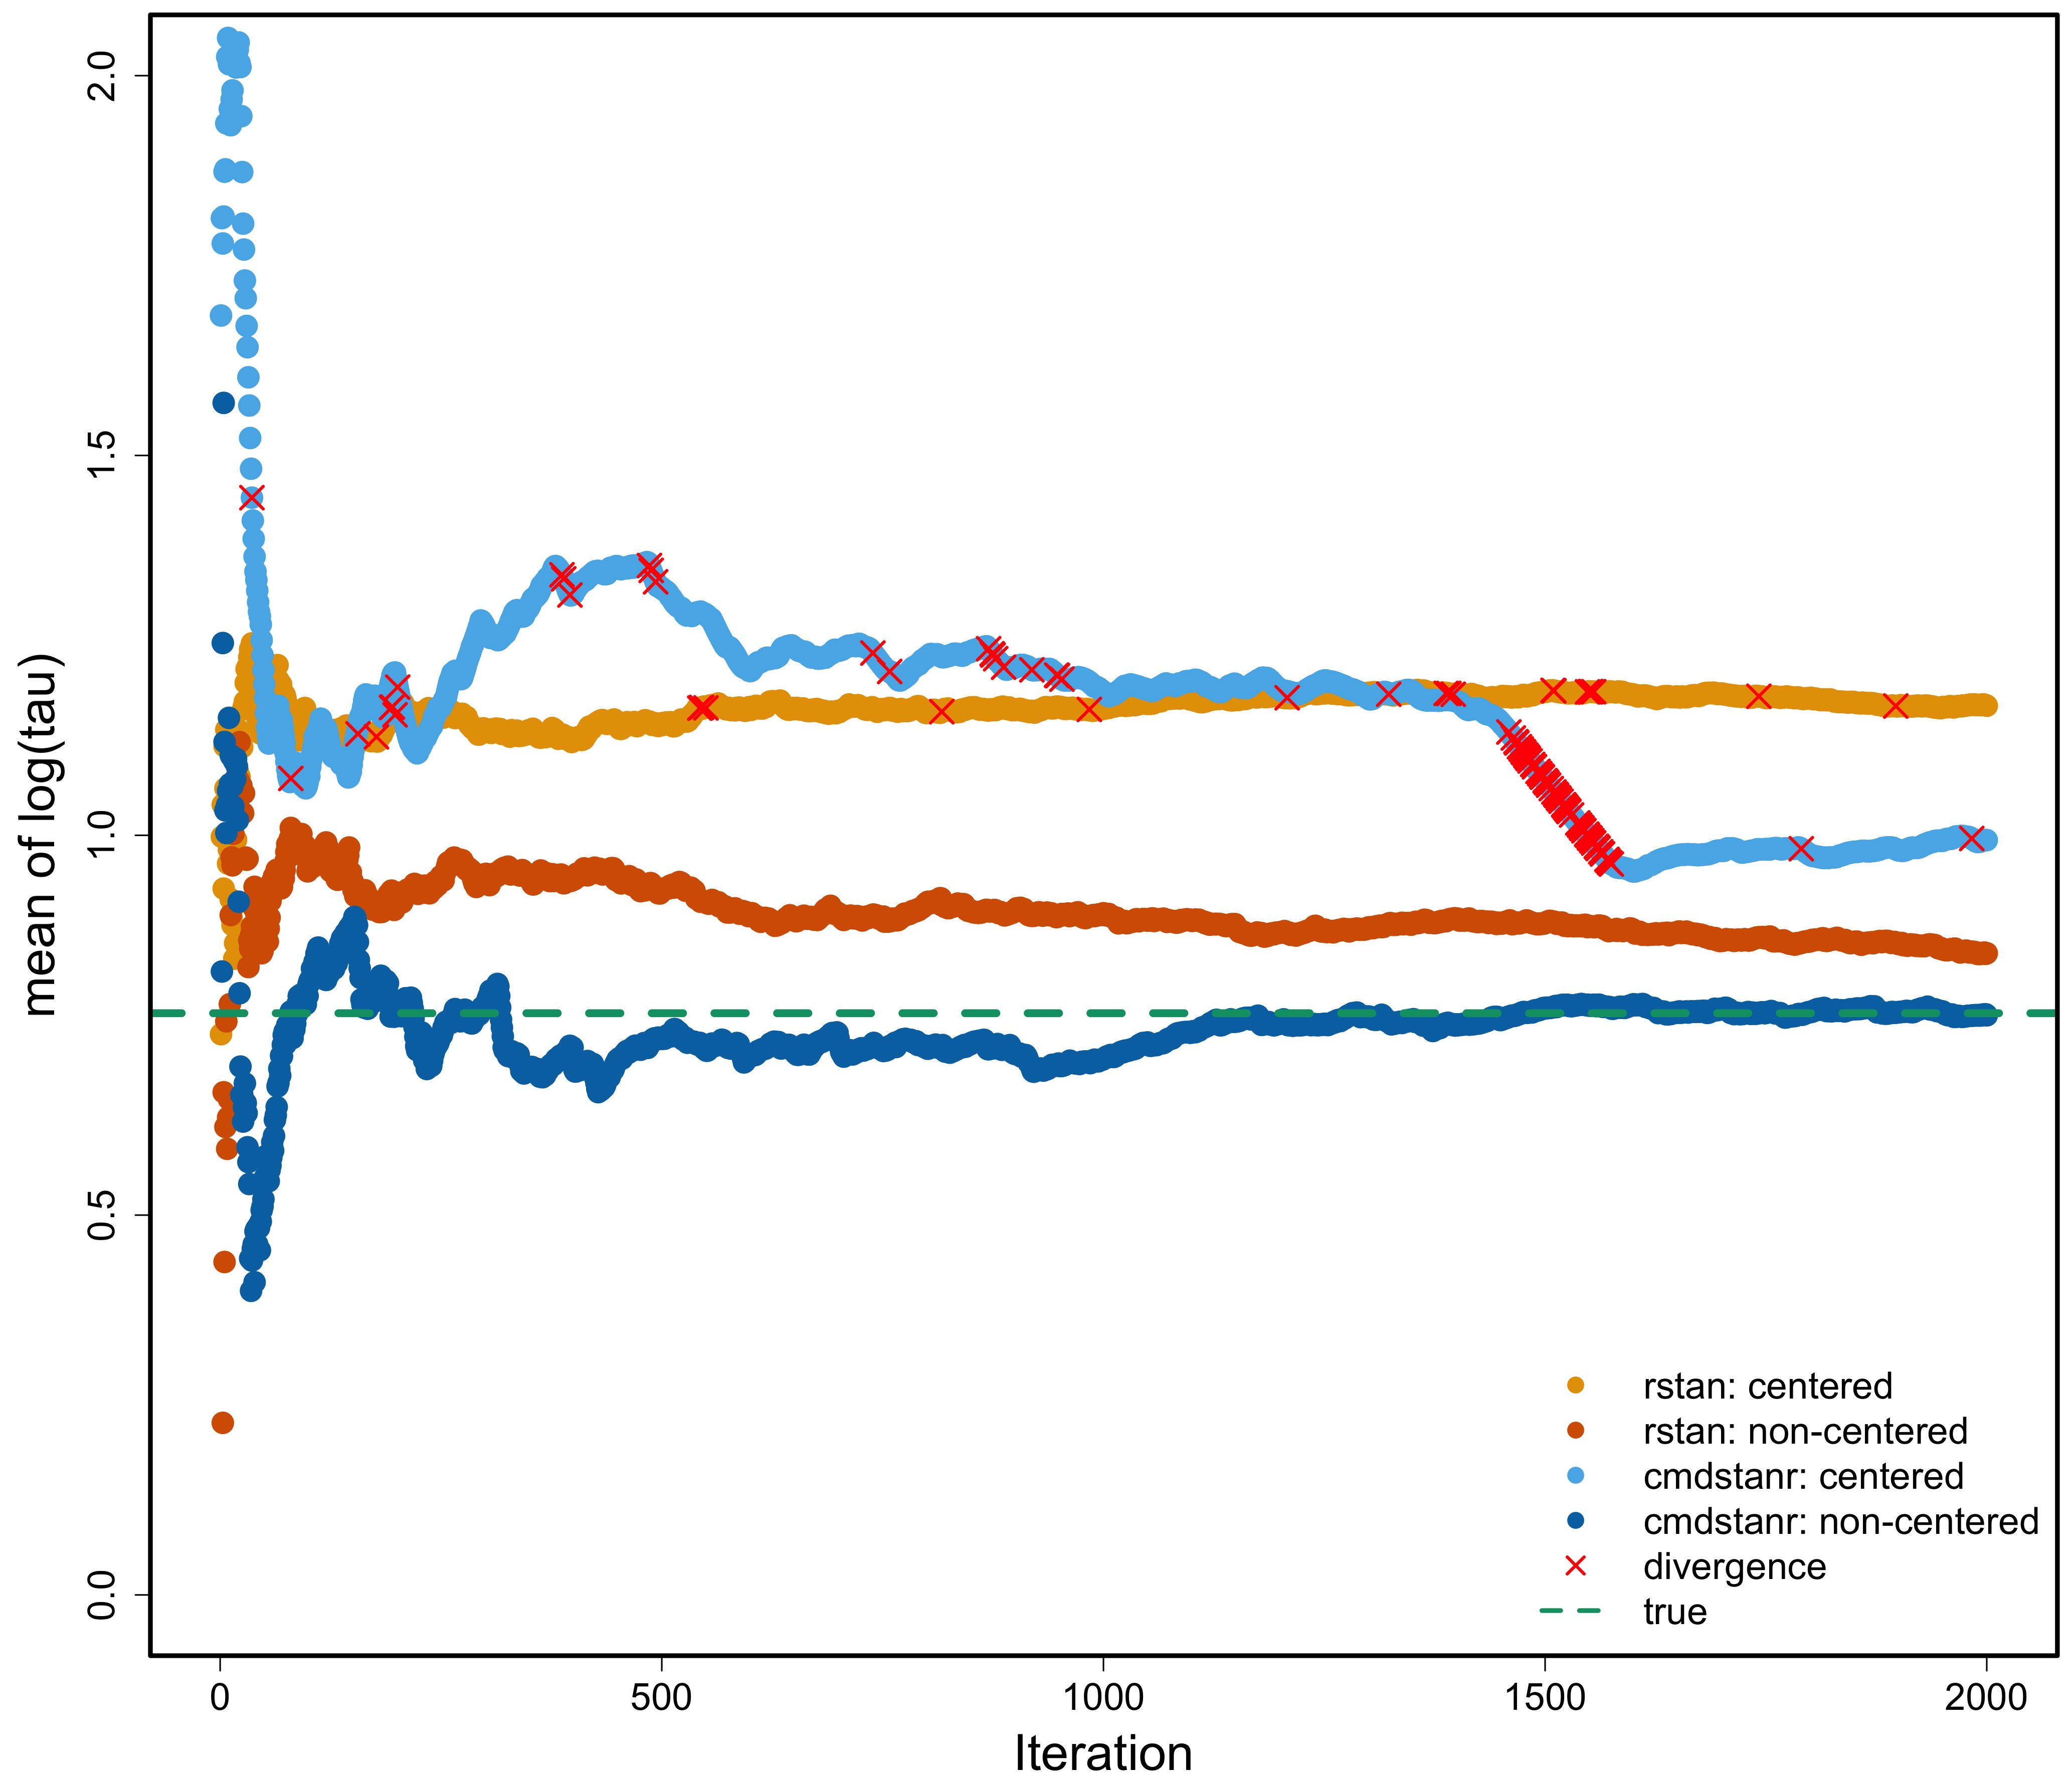
\includegraphics[width=0.9\textwidth]{Figures/Chp1_mean_tau.jpg}
\caption{Convergence of mean $log(\tau)$ towards the true expected value across four scenarios}
\label{fig:chp1_mean_tau}
\end{figure}

\begin{figure}[H]
\centering
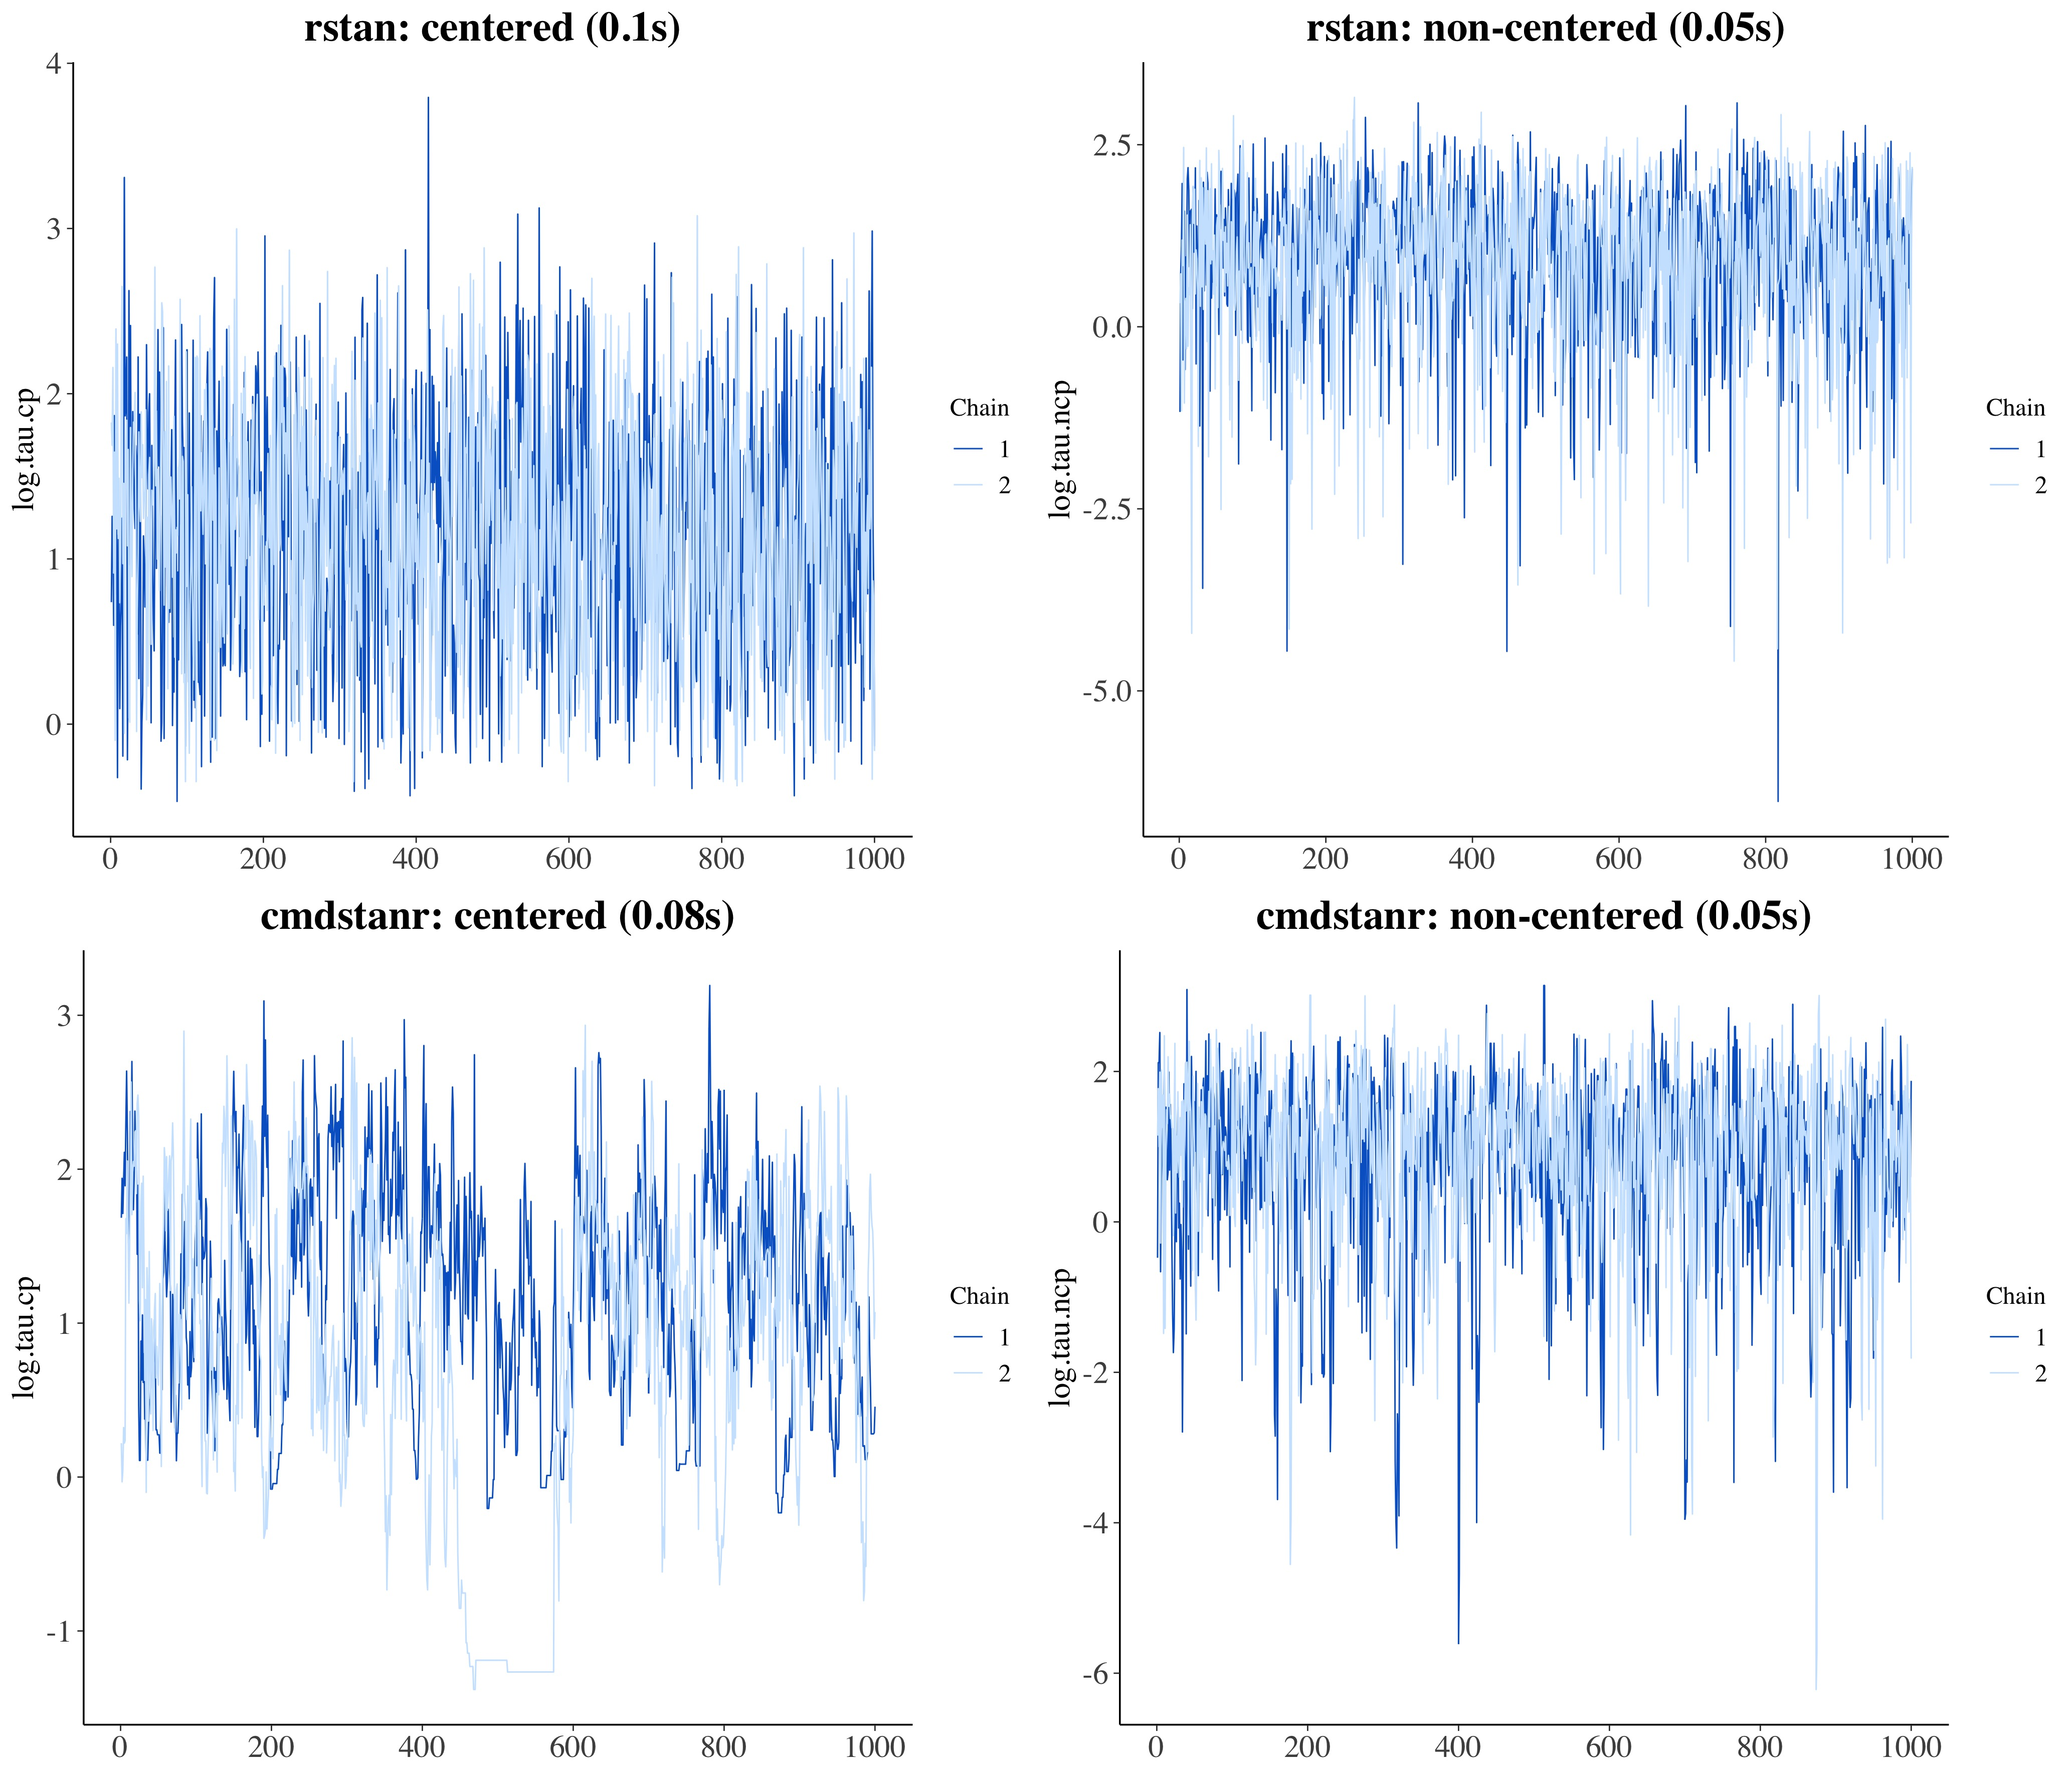
\includegraphics[width=\textwidth]{Figures/Chp1_trace_tau.jpg}
\caption{Trace plot of $log(\tau)$ across four scenarios with elapsed time in parentheses}
\label{fig:chp1_trace_tau}
\end{figure}







